\chapter{Background}


\section{The Wind Farm Layout Optimization Problem}


\textit{Finding the number of wind turbines, and position for each wind turbine relative to each other to maximize the expected power production within a given budget.}\\


\noindent Installing wind turbines in wind farms, reduces both installation and maintenance costs. In spite of this advantage, installing wind turbines in a farm also has its disadvantages. When wind turbines are placed together, the speed that hits a turbine will be reduced by a wake of turbulence generated by turbines that are in front of it. This effect is called the wake effect, and will be discussed more thoroughly later. If not considered, the wake effect can lead to extensive power loss. Therefore, it is crucial to find a positioning of the turbines that reduces the wake effect. The wind farm layout optimization problem is the problem of finding the optimal number of turbines to be positioned, and the optimal position for the turbines relative to each other. The goal is to find a layout the produces a maximal amount of expected power within a given budget.


\section{Genetic Algorithm (GA)}


% Reference Holland (inventor)
% Reference Darwin (evolution)
% Reference Goldberg (description)


% Why GA
Genetic algorithms are probabilistic search algorithms inspired by natural selection and survival of the fittest. They operate on complex problems that would be very difficult, maybe even impossible, to solve by classical methods. Genetic algorithms are very robust and can find near-optimal solutions to problems without knowing anything about how an optimal solution look like, they only require a method of measuring the "goodness" or fitness of a solution.


% How GA works
Genetic algorithms work as follows: An initial population of individual solutions is generated and the fitness of each individual is calculated based on a fitness function, which from now on will be called an objective function. Based on their objective function values the fittest individuals are selected for reproduction. By combining genes of the parent solutions and perform genetic operations such as mutation, a new pool of solutions is generated. Since the solutions of the newly generated population is produced by recombining the fittest solutions from the initial population the average fitness of the newly generated population is expected to be higher than the one of the initial population. This process continues until some stopping condition is reach, and by then the average and best fitness of the population should be pretty high. Figure \ref{GA Flow chart} shows the main operations of the genetic algorithm.


% Figure of GA
\begin{figure}[h!]
\begin{center}
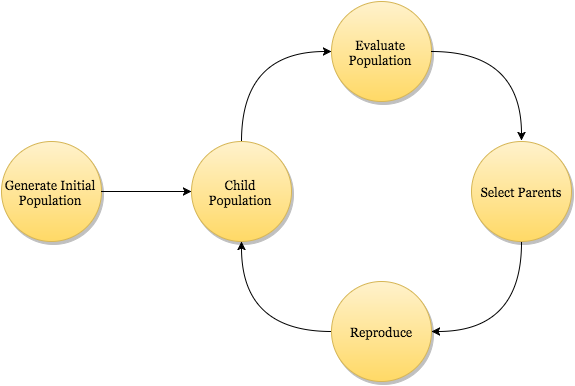
\includegraphics[scale=0.5]{images/GA}
\caption{The main operations of and genetic algorithm}
\end{center}
\label{GA Flow chart}
\end{figure}


% Representation
%\subsubsection{Representation of individuals and Reproduction}
%The individuals (solutions) that the GA perform operations on are represented as bit-strings. Initially each bit-string is generated by randomly assigning either zero or one to each of the ''genes'' of the individual. An example of an individual is given below:
%
%
%\begin{figure}[h!]
%    \centering
%    \begin{subfigure}[b]{0.3\textwidth}
%        \includegraphics[width=\textwidth]{"Single Point Crossover"}
%        \caption{Single-point crossover.}
%        \label{fig:gull}
%    \end{subfigure}
%    ~ %add desired spacing between images, e. g. ~, \quad, \qquad, \hfill etc. 
%      %(or a blank line to force the subfigure onto a new line)
%    \begin{subfigure}[b]{0.3\textwidth}
%        \includegraphics[width=\textwidth]{"Double Point Crossover"}
%        \caption{Double-point crossover.}
%        \label{fig:tiger}
%    \end{subfigure}
%    \caption{Crossover operations. (a) Singe point crossover at position four. (b) Double-point crossover at positions three and nine.}\label{fig:animals}
%\end{figure}


\subsection{The Island Model}
The island model is an extension of the general GA where the initial population of size $N_{total}$ is partitioned into $N_{island}$ such that each island holds a population of size $N_{total} / N_{island}$. The separated populations can then evolve on each island, exploring different solutions, until a migration takes place. A migration is when some individuals from one island migrate to another island. Figure \ref{Island Model} shows an island model consisting of four island where the arrows shows legal migration routes. The topology of the island network and migration routes can take many different forms. 

The advantage of using the island model, as compared to the classical GA is that in the classical GA the population can converge to a non-optimal solution quite fast, because a few individuals can take over the entire population and guide it towards a sub-optimal solution. Using the island model the probability of converging to a sub-optimal solution will decrease because each island can investigate a different part of the solution space. 


\begin{figure}[h!]
\begin{center}
\includegraphics[scale=0.5]{images/"Island Model"}
\caption{Island Model}
\end{center}
\label{Island Model}
\end{figure}


\subsection{The Cellular Model}


\begin{figure}[h!]
\begin{center}
\includegraphics[scale=0.5]{images/"Cellular Model"}
\caption{Cellular Model}
\end{center}
\label{Cellular Model}
\end{figure}


\section{Wind Farm Layout Optimization using Genetic Algorithms}

% Mosetti et al, 1994
In 1994, Mosetti et al. successfully utilized the genetic algorithm on the wind farm layout optimization problem \textcolor{red}{[Mosetti et al., 1994]}. To model the wind decay Mosetti et al. used a model similar to the Jensen model \textcolor{red}{[Jensen, 1983]}. Mosetti et al. divided the wind farm terrain into a $10\times10$ quadratic grid so that a wind turbine could be installed in the middle of each cell. The optimization problem would then be to find which cells wind turbines should be installed in, in order to maximize power production and minimize cost. With this representation, an individual of the genetic search could be represented as a binary string of length 100, where each index represents a cell in the grid, so that a value of 1 means that an wind turbine is installed in the corresponding cell, and a value of zero means that there is no wind turbine in the corresponding cell. The genetic algorithm used was a simple, single-population genetic search where the fittest individuals where selected for reproduction using crossover and mutation. The crossover operation was performed at random locations with probability $0.6 < P_c < 0.9$ and mutation was performed with probability $0.01 < P_m < 0.1$. The fitness of the individuals was determined by the objective function

\begin{equation}
Objective = \frac{1}{P_{total}}w_1 + \frac{cost_{total}}{P_{total}}w_2
\label{Objective function Mosetti et al.}
\end{equation}

where $P_{total}$ is the total energy produced in one year, $cost_{total}$ is a function of the number of wind turbines installed, and $w_1$ and $w_2$ are weights. In the current study, $w_1$ was kept small so that the focus would be on lowest cost per energy produced. The model was tested on a single type of turbines in three different scenarios (a) constant wind direction and intensity, (b) constant wind intensity, but from a 360$^{\circ}$ variable direction, and (c) a realistic wind scenario. This work laid the foundation for a number of studies of wind farm optimization using genetic algorithms. The genetic algorithms have been optimized, and they now run on much more realistic wind scenarios, cost-, and power models.\\

% Huang
\noindent Huang improved the results of Mosetti et al. by using a distributed genetic algorithm \textcolor{red}{[Huang, 2007]}. Huang stated that using a distributed genetic algorithm will not only decrease the computation time by using parallelism, but also achieve higher fitness because more of the solution space will be explored. The distributed algorithm distributed the population of 600 individuals among 20 demes, using a ring-topology as shown in figure \ref{Ring Topology}.

\begin{figure}[h!]
\begin{center}
\includegraphics[scale=0.3]{images/"Ring Topology"}
\caption{Ring topology example with 6 demes \textcolor{red}{[Huang, 2007]}.}
\label{Ring Topology}
\end{center}
\end{figure}


The simulation was run for 2500 generations with the migration strategy that 3.3\% of the individuals with highest fitness was selected as migrants, to replace the individuals with lowest fitness in the new population every 20th generation. \\

% Gao et al.
\noindent In 2015, Gao et al. used a distributed genetic algorithm to solve the wind farm optimization problem \textcolor{red}{[Gao et al., 2015]}. Unfortunately, they have kept most the implementation details of the distributed genetic algorithm to themselves, but they introduce an interesting hypothetical case study of wind turbine placement on an offshore farm located in the Hong Kong southeastern water. By using real wind data, collected over 19 years, they demonstrates that the distributed genetic algorithm can be applied to a real-world wind farm layout optimization problem. It should also be noted that Gao et al. do not use the constraint that the turbines have to be positioned in the middle of a cell. This property is made possible by inspecting the positions of the turbines relative to each other, and reassign the turbines that are too close to other positions \textcolor{red}{They borrowed this method from Wan et al., 2009}.\\

% Sisbot et al.
\noindent \c{S}i\c{s}bot et al. published a case study of wind turbine placement on a wind farm at the Island G{\"o}k\c{c}eada, at the north east of the Aegean Sea \textcolor{red}{[\c{S}i\c{s}bot et al., 2010]}. A distributed genetic algorithm was used, but, unlike Huang, the individuals were evaluated based on multiple objective functions; one that measures the total cost (installation and operational), and one that measure total power production. \c{S}i\c{s}bot et al. argue that in an environment with changing demands, the use of a multi-objective function gives the decision-makers the opportunity to evaluate the different designs based on cost and power production separately, without ill-informed, randomly generated weights.

The selection process used is a controlled, elitist process, meaning that not only the fittest, but also some individuals that can spread diversity to the population are selected for reproduction. The genetic algorithm returns a set of Pareto optimal solutions; a set of solutions that are not dominated by any other solution in the set. Stated more formally, solutions \textbf{y} is said to dominate solution \textbf{x} if

\begin{equation}
\forall i: f_i(\textbf{x}) \leq f_i(\textbf{y}) \hspace{1mm} and \hspace{1mm} \exists j: f_j(\textbf{x}) < f_j(\textbf{y}) 
\label{Dominated solutions}
\end{equation}

where $f_i$ is objective function \textcolor{red}{[Murata et al., 2001]}. Other interesting features of this study is the introductions of constraints on wind turbine positions and constraints on the cost, meaning that individuals with wind turbines outside the area of the island, and individuals with costs larger than the budget are removed from the population. Even thought constraints on individuals are not in accordance with the nature genetic algorithms, they can be necessary when the algorithm is applied to a real problem. Another feature introduced in this paper is rectangular cells. The argument behind this decision is that the safe distance between wind turbines is dependent of the direction of the turbine. The minimum distance between turbines in prevailing wind is 8D, while the minimum distance between turbines in the crosswind is 2D. In spite of this attempt to make the wind scenario more realistic, it is critiqued because it operates with a constant wind direction and constant speed, using the average wind direction and speed measured at the Island \textcolor{red}{[Samorani, 2013]}. \\